%%%%%%%% ICML 2018 EXAMPLE LATEX SUBMISSION FILE %%%%%%%%%%%%%%%%%

\documentclass{article}

% Recommended, but optional, packages for figures and better typesetting:
\usepackage{amsmath, amssymb}
\usepackage{mathtools}
\usepackage{microtype}
\usepackage{graphicx}
\usepackage{subfigure}
\usepackage{booktabs} % for professional tables
\usepackage{xcolor}
\usepackage{algorithmic}

% hyperref makes hyperlinks in the resulting PDF.
% If your build breaks (sometimes temporarily if a hyperlink spans a page)
% please comment out the following usepackage line and replace
% \usepackage{icml2018} with \usepackage[nohyperref]{icml2018} above.
\usepackage{hyperref}

%! TEX root = main.tex
\usepackage{xcolor}
\usepackage{algorithm}
\usepackage{algpseudocode}
\usepackage{hyperref}

%\newcommand{\deltat}{\delta\hspace*{-.3mm}t}
\newcommand{\deltat}{\ensuremath{\delta\hspace{-.06em}t}}
\newcommand{\bigO}[1]{O (#1)}
\newcommand{\reward}{\tilde{r}}
\newcommand{\actionspace}{\mathcal{A}}
\newcommand{\statespace}{\mathcal{S}}
\newcommand{\NDC}[1]{\color{red}NDC:#1\color{black}}

\newcommand{\pfield}{\mathcal{F}_t}
\newcommand{\Ep}[1]{\BE\left[#1\mid\pfield\right]}
\newcommand{\diag}[1]{\mathrm{\textbf{diag}}(#1)}
\newcommand{\lmax}{\lambda_{\mathrm{max}}}



\newcommand{\mynumero}{n°}


%\def\d{{\mathrm{d}}}
%\def\d{\operatorname{d}\!}
\def\d{\operatorname{d}\!{}}
%\def\d{\operatorname{}\!\mathrm{d}}

\def\N{{\mathbb{N}}}
\def\Z{{\mathbb{Z}}}
\def\Nstar{{\mathbb{N}^\star}}
\def\Q{{\mathbb{Q}}}
\def\R{{\mathbb{R}}}
\def\C{{\mathbb{C}}}

\renewcommand{\geq}{\geqslant}
\renewcommand{\leq}{\leqslant}

\renewcommand{\emptyset}{\varnothing}

\newcommand{\deq}{\mathrel{\mathop{:}}=}
\newcommand{\eqd}{=\mathrel{\mathop{:}}}

\newcommand{\from}{\colon} % correct ':' in f\from X \to Y
\newcommand{\st}{\mid} % set builder
%\newcommand{\st}{\mathrel{}\middle|\mathrel{}} % set builder

\def\eps{\varepsilon}
\renewcommand{\epsilon}{\varepsilon}
\renewcommand{\phi}{\varphi}

\def\ds{\displaystyle}

\DeclareMathOperator{\dist}{dist}
\DeclareMathOperator{\diam}{diam}
\DeclareMathOperator{\vol}{vol}
\DeclareMathOperator{\Ric}{Ric}

\DeclareMathOperator{\lap}{\Delta\!}
\DeclareMathOperator{\nab}{\nabla\!\!}
\DeclareMathOperator{\Hess}{Hess}

\DeclareMathOperator{\Ent}{Ent}
\DeclareMathOperator{\Var}{Var}
\DeclareMathOperator{\Cov}{Cov}
\let\oldPr\Pr
\renewcommand{\Pr}{\oldPr\nolimits}
\newcommand{\E}{\mathbb{E}}
\newcommand{\KL}[2]{\mathrm{KL}\!\left(#1 \,|\hspace{-.15ex}|\,#2\right)}

\DeclareMathOperator{\mult}{mult}
\DeclareMathOperator{\Card}{Card}
\DeclareMathOperator{\Aut}{Aut}
\DeclareMathOperator{\Epi}{Epi}
\DeclareMathOperator{\Spec}{Sp}
%\DeclareMathOperator{\Ker}{Ker}
\DeclareMathOperator{\Img}{Im}
\DeclareMathOperator{\Tr}{Tr}
\DeclareMathOperator{\tr}{tr}
\DeclareMathOperator{\Tor}{Tor}
\DeclareMathOperator{\Ext}{Ext}
\DeclareMathOperator{\Hom}{Hom}
\DeclareMathOperator{\End}{End}
\DeclareMathOperator{\coker}{coker}
\DeclareMathOperator{\Id}{Id}
\DeclareMathOperator{\id}{id}
%\DeclareMathOperator{\diag}{diag}


\newcommand{\abs}[1]{\left\lvert#1\right\rvert}
\newcommand{\norm}[1]{\left\lVert#1\right\rVert}
\newcommand{\scal}[2]{\left< \, #1 \mid #2 \, \right>}
\newcommand{\1}{\mathbbm{1}}

\newcommand{\ilim}[1]{\underset{#1}{\underrightarrow{\lim\vspace{.5ex}}}\,}
\newcommand{\plim}[1]{\underset{#1}{\underleftarrow{\lim\vspace{.5ex}}}\,}

\DeclareMathOperator*{\vlimsup}{\varlimsup}
\DeclareMathOperator*{\vliminf}{\varliminf}

\newcommand{\presgroup}[2]{\left\langle\,#1 \mid  #2\,\right\rangle}

\newcommand{\twopi}{2\hspace{-.23em}\pi}

%\DeclareMathOperator*{\argmax}{arg\,max}
%\DeclareMathOperator*{\argmin}{arg\,min}



% Use the following line for the initial blind version submitted for review:
\usepackage{icml2018}

% If accepted, instead use the following line for the camera-ready submission:
%\usepackage[accepted]{icml2018}

% The \icmltitle you define below is probably too long as a header.
% Therefore, a short form for the running title is supplied here:
\icmltitlerunning{Deep Relativistic Advantage Updating}

\begin{document}

\twocolumn[
\icmltitle{There are no small Advantages:
	Reinforcement learning in near continuous time
	with Deep RelAtive Mixture of Advantages
}


% It is OKAY to include author information, even for blind
% submissions: the style file will automatically remove it for you
% unless you've provided the [accepted] option to the icml2018
% package.

% List of affiliations: The first argument should be a (short)
% identifier you will use later to specify author affiliations
% Academic affiliations should list Department, University, City, Region, Country
% Industry affiliations should list Company, City, Region, Country

% You can specify symbols, otherwise they are numbered in order.
% Ideally, you should not use this facility. Affiliations will be numbered
% in order of appearance and this is the preferred way.
\icmlsetsymbol{equal}{*}

\begin{icmlauthorlist}
%\icmlauthor{Aeiau Zzzz}{equal,to}
%\icmlauthor{Bauiu C.~Yyyy}{equal,to,goo}
%\icmlauthor{Cieua Vvvvv}{goo}
%\icmlauthor{Iaesut Saoeu}{ed}
%\icmlauthor{Fiuea Rrrr}{to}
%\icmlauthor{Tateu H.~Yasehe}{ed,to,goo}
%\icmlauthor{Aaoeu Iasoh}{goo}
%\icmlauthor{Buiui Eueu}{ed}
%\icmlauthor{Aeuia Zzzz}{ed}
%\icmlauthor{Bieea C.~Yyyy}{to,goo}
%\icmlauthor{Teoau Xxxx}{ed}
%\icmlauthor{Eee Pppp}{ed}
\end{icmlauthorlist}

%\icmlaffiliation{to}{Department of Computation, University of Torontoland, Torontoland, Canada}
%\icmlaffiliation{goo}{Googol ShallowMind, New London, Michigan, USA}
%\icmlaffiliation{ed}{School of Computation, University of Edenborrow, Edenborrow, United Kingdom}
%
%\icmlcorrespondingauthor{Cieua Vvvvv}{c.vvvvv@googol.com}
%\icmlcorrespondingauthor{Eee Pppp}{ep@eden.co.uk}

% You may provide any keywords that you
% find helpful for describing your paper; these are used to populate
% the "keywords" metadata in the PDF but will not be shown in the document
\icmlkeywords{Reinforcement learning}

\vskip 0.3in
]

% this must go after the closing bracket ] following \twocolumn[

% This command actually creates the footnote in the first column
% listing the affiliations and the copyright notice.
% The command takes one argument, which is text to display at the start of the footnote.
% The \icmlEqualContribution command is standard text for equal contribution.
% Remove it (just {}) if you do not need this facility.

%\printAffiliationsAndNotice{}  % leave blank if no need to mention equal contribution
%\printAffiliationsAndNotice{\icmlEqualContribution} % otherwise use the standard text.

\begin{abstract}
	Despite remarkable successes, \emph{Deep Reinforcement learning} remains sensitive to
	hyperparameterization, implementation details and small environment changes~(\citealt{drl_matter}, \citealt{drl_matter_bis}). 
	Overcoming this sensitivity is key to making DRL applicable to real world problems.
	In this paper, we study the sensitivity of Deep Reinforcement learning algorithms to
	time discretization. More precisely, we show that approaches based on estimations of the
	Q-function, e.g. \emph{Deep Q-learning}~\cite{dqn} and \emph{Deep deterministic policy gradient}~\cite{ddpg}
	are sensitive to variations of time discretization. We further show that a simple reparameterization of the
	Q-function as a sum of a state value term and a \emph{small} action dependent advantage term yields an algorithm
	much more resilient to variations of time discretization.
\end{abstract}

\section{Introduction}
\label{sec:intro}
In recent years, deep learning based approaches to reinforcement learning have
thrived and provided impressive results in a variety of domains, achieving superhuman
performances with no expert knowledge in perfect information zero-sum
games~\cite{alphazero}, reaching level of top players in video
games~(\citealt{openai_five}, \citealt{dqn}), or learning dexterous manipulation
from scratch without demonstrations~\cite{hand_control}.

In spite of those successes, \emph{Deep reinforcement learning} approaches are
sensitive to a number of factors, including hyperparameterization,
implementation details or small changes in the environment
parameters~(\citealt{drl_matter}, \citealt{drl_matter_bis}). This sensitivity,
along with sample inefficiency, prevents DRL from being applied in most real
world settings. High sensitivity to environment parameters notably prevents
transfering abilities from imperfect simulators to real world scenarios.

In this paper we focus our attention on the sensitivity to time discretization
of DRL approaches, i.e. what happens when an agent receives $50$ observations
and is expected to take $50$ actions per second instead of $10$. One expects
that decreasing time discretization, or equivalently shortening reaction time,
should only improve agent performances. This is not what happens in practice
for approaches based on estimation of state action value functions, e.g.
\emph{Deep Q-learning} (DQN~\citep{dqn} and \emph{Deep deterministic policy
gradient} (DDPG~\citep{ddpg}). This is shown experimentally in Sec.~\ref{sec:exp}.

We relate this sensitivity to the fact that, as the discretization timestep
decreases, the effect of individual actions on the total return decreases, and
can vanish when the discretization timestep becomes infinitesimal. The natural
framework to study this phenomenon is Continuous time reinforcement learning 
(Sec.~\ref{sec:continous}). 

To cope for this effect, we introduce a
parameterization of the Q-function as a sum of a state value term and a
\emph{small} action dependent advantage term (Sec.~\ref{subsec:reparam}). This
reparameterized Q approximation can be trained with deep variants of Q-learning
(Sec.~\ref{subsec:algorithm}).  To properly scale w.r.t. time discretization,
particular attention has to be taken regarding both the exploration method, and
the scaling of learning rates (Sec.~\ref{subsec:lr}, Sec.~\ref{subsec:explo}).
The resulting algorithm is shown to provide near perfect invariance to time
discretization on simple environments, and much better invariance properties
than vanilla DQN or DDPG on more complex environments (Sec.~\ref{sec:exp}).

\section{Related work}
\label{sec:related}
Continuous and near continuous reinforcement learning, which is at the core of
our approach has been thoroughly studied in the deterministic case
in~\cite{adv_upd} or \cite{cont_rl}, but has not been applied in the context of
deep reinforcement learning.

The approach presented in this paper is closely related to \cite{adv_upd} and
\cite{cont_rl}. \cite{adv_upd} already separated the learning procedure of the
value and advantage functions, and introduced proper scalings between the two
components. We extend on \cite{adv_upd} in three directions. We provide a
formal argument on why the advantage contribution of the Q-function is of order
$\bigO(\deltat)$, irrelevant of the stochasticity of the environment, in a quite
general framework. We show that, provided with well suited learning rates and
exploration method, Advantage updating provide near invariance to change of time
discretization. We show that Advantage updating is viable in the context of deep
reinforcement learning, while not using the true gradient of the residual error.

More recently, \cite{dueling_nets} also introduced a parameterization separating
the value and the advantage components of the Q-function. We additionally
introduce a natural scaling coeficient between the two, that strongly improves
the time discretization invariance properties.

\section{Near continuous time reinforcement learning}
\label{sec:continous}
% In this section, a continuous reinforcement learning framework is introduced,
% and it is shown that under this framework, the state-action value function does
% not depend on the action. We further show that in near continous domains, when
% the discretization timestep $\deltat$ is small, the difference in state-action
% value between two different actions in a fixed state is of order $\bigO(\deltat)$.
TODO. Main ideas: near continuous time environments (control, mujoco, video games, ...)
There is a time discretization $\deltat$ given by the problem. The uderlying process does not depend of $\deltat$. Need to see what is happening when changing $\deltat$. The problem is invariant to $\deltat$. The quantities we are looking at should be invariant to. The learning procedure should be invariant. Looking at the limits when $\deltat \rightarrow 0$. In simulated environments, changing $\deltat$ only means to change the FPS. In real environments, for example with robots, this could mean changing the quality of the sensors and motors.

\subsection{Framework}

Let assume that we have a Markov Decision Process (TODO:Cite?) $\langle {\cal S}, {\cal A}, T_{\deltat}, r, \gamma\rangle$. ${\cal S}$ is the state-space, which is supposed to be continuous (TODO:not the good formulation). The action space is TODO.

We assume that the transition is continuous. This means that ... TODO. Discussion on the hypothesis, in which environments it is true. Is the condition $\forall \deltat, \forall s, \E[\|s_{k+1} - s_k \||s_k = s] \leq ?$. 

In what follows, $\dt$ denotes a truly infinitesimal time interval while $\deltat$
denotes a small, but non infinitesimal time interval. Similarily, $\dbt$ denotes
an infinitesimal (multi-dimensional) brownian step, while $\deltabt$ denotes its
discretized equivalent. Informally, $\dbt$ is to be thought of as $\gauss(0, \sqrt{\dt}^2)$,
and $\deltabt$ as $\gauss(0, \sqrt{\deltat}^2)$, where $\gauss(\mu, \sigma)$ denotes a gaussian
random variable of mean $\mu$ and standard deviation (or covariance matrix in the multi-dimensional case)
$\sigma$.

Consider a fully observable \emph{Markov Decision Process} defined by the following
transitions and rewards
\begin{align}
	ds(s, a) &= F(s, a) dt + \Sigma(s, a) \dbt\\
	dr(s, a) &= \reward(s, a) dt + \Sigma_r(s, a) \dbt.
\end{align}
The equation on $s$ is that of a diffusion process, with drift coeficient $F$
and diffusion matrix $\Sigma$.  This framework is only moderately restrictive.
For example, deterministic continuous control environments fall in this
framework, with $\Sigma = 0$ and $\Sigma_r = 0$. Limitations of the framework
are discussed in Sec.~\ref{sec:discussions}.
This framework is naturally discretized to arbitrary $\deltat$ by replacing all
$d$'s with $\delta$'s.

A continuous policy $\pi$ is defined as a deterministic mapping from states to
actions.  In continuous time, defining stochastic policies with well defined
state-value functions requires incorporating information from previous action into
the state to obtain a temporally coherent policy. To avoid such inconvenience, the
framework is restricted to deterministic policies. This is a mild constraint, as this
only enforces determinism of the exploitation policy and not of exploration policies.
In what follows, $\tau\sim\pi$ denotes a trajectory of states and actions sampled
according to policy $\pi$, with $s_0$ sampled according to an arbitrary initial distribution
on states $\rho_0$, and $dr_{t} = dr(s_t, a_t)$.

Under a deterministic policy $\pi$, one can define the $\gamma$ discounted
\emph{state value function} $V^\pi(s)$ and \emph{state action value function}
$Q^\pi(s, a)$ as
\begin{align}
	V^\pi(s) &= \E_{\tau\sim\pi}\left[
		\int\limits_{t=0}^\infty \gamma^{t}
		dr_{t} \mid s_0 = s
	\right]\\
	Q^\pi(s, a) &= \E_{\tau\sim\pi}\left[
		\int\limits_{t=0}^\infty \gamma^{t}
		dr_{t} \mid s_0 = s, a_0 = a
	\right]
\end{align}
which are naturally discretized as
\begin{align}
	V^\pi(s) &= \E_{\tau\sim\pi}\left[
		\sum\limits_{k=0}^\infty \gamma^{k\deltat}
		\delta r_{k\deltat} \mid s_0 = s
	\right]\\
	Q^\pi(s, a) &= \E_{\tau\sim\pi}\left[
		\sum\limits_{k=0}^\infty \gamma^{k\deltat}
		\delta r_{k\deltat} \mid s_0 = s, a_0 = a
	\right].
\end{align}
Both $V^\pi$ and $Q^\pi$ verify Bellman equations, informally
\begin{align}
	V^\pi(s) &= \reward(s, \pi(s))\dt + \gamma^{\dt} \E_{ds \sim ds(s, \pi(s))} V^\pi(s + ds)\nonumber\\
	Q^\pi(s, a) &= \reward(s, a)\dt + \gamma^{\dt} \E_{ds(s, a)} V^\pi(s + ds(s, a))
	\label{eq:cont_bell}
\end{align}
which in continuous time translates, using Ito's lemma, into a Hamilton Jacobi equation
\begin{align}
	\reward + \partial_s V^\pi \cdot f + \frac{1}{2} \text{tr}\left(\Sigma^T\partial^2_{s^2} V^\pi\Sigma\right) = (1 - \gamma) V^\pi(s).
\end{align}

\subsection{Independence of $Q^\pi$ on $a$ in continuous time}
Consider a discretization of Eq.~\eqref{eq:cont_bell} with time interval
$\deltat \ll~1$, Ito's lemma yield
\begin{align}
	Q^\pi(s, a) &= \reward(s, a) \deltat + \gamma^{\deltat} \E_{\delta s \sim \delta s(s, a)}V^\pi(s + \delta s)\nonumber\\
		    &= \reward(s, a) \deltat + \gamma^{\deltat} V^\pi(s) +
		     \gamma^{\deltat} \partial_s V^\pi(s)f(s, a) \deltat\nonumber\\
		    &+ \frac{1}{2}\text{tr}\left(\Sigma^T\partial^2_{s^2}V^\pi(s)\Sigma\right)\deltat + \bigO(\deltat^2)\nonumber\\
		    &\xrightarrow[\deltat \to 0]{} V^\pi(s).
		    \label{eq:Q_cont}
\end{align}
A consequence of Eq.~\eqref{eq:Q_cont} is that in exact continuous time,
$Q^\pi$ does not bear any information on the hierarchy of actions, and
thus cannot be used to select actions that yields higher future returns.

As the difference between between $Q^\pi(s, a)$ and $V^\pi(s)$ is of order
$\bigO(\deltat)$, it is natural to define a rescaled version of the advantage
function, namely
\begin{align}
	A^\pi(s, a) &= \frac{Q^\pi(s,a) - V^\pi(s)}{\deltat}\\
		    &= \reward(s, a) +
		    \frac{\gamma^{\deltat} \E_{\delta s \sim \delta s(s, a)} V^\pi(s + \delta s) - V^\pi(s)}{\deltat}.
    \label{eq:adv}
\end{align}
Contrary to the action state value function, the rescaled advantage function converges
to an action dependent quantity when $\deltat$ goes to $0$
\begin{align}
	A^\pi(s, a) &\xrightarrow[\deltat \to 0]{} \reward(s, a) +
	(\gamma - 1) V^\pi(s) + \partial_s V^\pi(s) f(s, a)\nonumber\\
		    &+
	\frac{\text{tr}\left(\Sigma^T(s, a)\partial^2_{s^2}V^\pi(s) \Sigma(s,a)\right)}{2},
\end{align}
and $Q^\pi$ can then be rewritten as
\begin{equation}
	Q^\pi(s, a) = V^\pi(s) + \deltat A^\pi(s, a).
	\label{eq:reparam_q_pi}
\end{equation}


%! TEX root = icml_drau.tex
\section{Reinforcement Learning with a Continuous-Time Limit}

We now define a discrete algorithm with a well-defined continuous-time
limit.  It relies on three elements: defining and learning a quantity
that still contains information on action rankings in the limit, using
exploration methods with a meaningful limit, and scaling learning rates
to induce well-behaved parameter trajectories when $\deltat$ goes to $0$.

% When the approximate $Q$-function is initialized, if the effect of
% actions on the $Q$-function is order of magnitudes higher than what it should be,
% approximating $Q^\pi_\deltat$ is likely to be difficult.
%Besides, the error is likely
%to be further propagated when the equation used to update our approximate $Q$
%function relies on bootstraping, as is the case for usual temporal difference
%derived methods.

\subsection{Advantage Updating}
\label{subsec:reparam}

As seen above, there is no continuous time limit to $Q$-learning, because
$Q^\pi$ becomes independent of actions and thus cannot be
used to select actions.  In near-continuous time,
$Q^\pi_\deltat$ still depends on actions, and could still be used to
choose actions. However, when
approximating $Q^\pi_\deltat$, if the approximation error is much larger
than $\bigO(\deltat)$, this error dominates, the ranking of
actions given by the approximated $Q^\pi_\deltat$ is likely to be erroneous.

To define an object which contains the same information on actions as
$Q^\pi_\deltat$, but admits a learnable action-dependent limit, it is
natural to define \cite{adv_upd}
\begin{align}
	A^\pi_\deltat(s, a) &\mathdef \frac{Q^\pi_\deltat(s,a) - V^\pi_\deltat(s)}{\deltat},
    \label{eq:adv}
\end{align}
a rescaled version of the advantage function, as the difference between between
$Q^\pi_\deltat(s, a)$ and $V^\pi_\deltat(s)$ is of order
$\bigO(\deltat)$. This amounts to splitting $Q$ into value and advantage,
and observing that these scale very differently when $\deltat\to 0$.

Contrary to the action state value function,
this
rescaled advantage function converges when $\deltat\to 0$
to an action-dependent quantity which, if it can be learned, contains the
necessary information for policy improvement (Thm.~\ref{thm:Alimit}).


% \LB{In next equation, tiny detail but I would write $\frac{1}{\deltat}(r\deltat+...)$, easier to read.}
% \begin{align}
% 	A^\pi_\deltat(s, a)=&\reward(s, a)+\frac{\gamma^{\deltat}\E_{\deltas \sim \deltas(s, a)}V^\pi_\deltat(s + \deltas)-V^\pi_\deltat(s)}{\deltat}\nonumber\\
% 	=&\reward(s, a)+\log(\gamma) V^\pi(s)+\partial_s V^\pi(s)f(s, a)\nonumber\\
%          &+\frac{\text{tr}\left(\Sigma^T(s, a)\partial^2_{s^2}V^\pi(s) \Sigma(s,a)\right)}{2} + O(\deltat)\nonumber.
% \end{align}

%   \begin{theorem}
%     There exists $A^\pi(s, a)$ such that for all $a, s$:
%     \begin{equation}
%       A^\pi_\deltat(s, a) \rightarrow_{\deltat \rightarrow 0} A^\pi(s, a)
%     \end{equation}
%     Moreover, $A^\pi$ contains all the necessary information for policy improvement. The policy $\pi$ optimal if and only if $A^\pi(s, \pi(s)) = \max_{a'}A^\pi(s, a')$ for all $s \in {\cal S}$.
%     \TODO{Is this true? What is true? Is this real life? We should probably add a reasonable hypothesis, for example $\pi_\deltat^* \rightarrow \pi^*$}
%   \end{theorem}

The discretized $Q$-function rewrites as
\begin{equation}
	Q^\pi_\deltat(s, a) = V^\pi_\deltat(s) + \deltat A^\pi_\deltat(s, a).
	\label{eq:reparam_q_pi}
\end{equation}
A natural way to approximate $V^\pi_\deltat$ and $A^\pi_\deltat$ is to apply
\emph{Sarsa} or $Q$-learning to a reparameterized $Q$-function approximator
\begin{equation}
	Q_\Theta(s, a) \deq V_{\theta}(s) + \deltat A_{\psi}(s, a).
\end{equation}
with $\Theta \deq (\theta, \psi)$. At initialization, if both $V_{\theta}$ and
$A_{\psi}$ are initialized independently of $\deltat$, this parameterization
provides reasonable scaling of the contribution of actions versus states
in $Q$.
Our goal is for $V_\theta$ to approximate $V^\pi_\deltat$ and for
$A_{\psi}$ to approximate $A^\pi_\deltat$.


%\TODO{CT and LB are fighting each other about the importance which should be given to the next paragraph. A impartial judge should give his opinion. (CT is wrong)}
Still, this reparameterization does not, on its own, guarantee that $A$
correctly approximates $A^\pi_\deltat$ if
$Q_\Theta$ approximates $Q^\pi_\deltat$% \footnote{
% 	Ensuring that $A$ does not differ from $A^\pi_\deltat$ by a state dependent function only affects
% 	$A$'s interpretability. Indeed, for any function $f$, the ranking of actions given by
% 	$A^\pi_\deltat(s, \cdot)$ and $A^\pi_\deltat(s, \cdot) + f(s)$ is
% 	the same. \TODO{still unclear why we'd care about identifiability}
%}
.
Indeed, for any given pair $(V_\theta,\,A_\psi)$, the pair $(V_\theta(s) -
f(s),\,A_\psi(s,a)+f(s)/\deltat)$ (for an arbitrary $f$)
% \begin{align}
% 	\tilde{V}(s) &= V(s) - f(s),\qquad
% 	\tilde{A}(s, a) = A(s, a) + \frac{f(s)}{\deltat}
% \end{align}
yields the exact same $Q_\Theta$ function. This new $A_\psi$ still defines %the same $Q$ and
the same ranking of actions, yet this phenomenon might cause
numerical problems or instability of $A_\psi$ when $\deltat\to 0$, and prevents direct
interpretation of the learned $A_\psi$.
% Consequently, $Q$ can correctly approximate
% $Q^\pi$ even if $A$ is arbitrarily far from $A^\pi$.
To enforce identifiability of $A_\psi$, one must enforce the consistency equation
\begin{equation}
	Q^\pi_\deltat(s, \pi(s)) - V^\pi_\deltat(s) = 0
\end{equation}
on the approximate $A_\psi$ and $V_\theta$. This translates to
\begin{equation}
	A_\psi(s, \pi(s)) = 0.
\end{equation}
With this additional constraint, if $Q_\Theta = Q^\pi_\deltat$, then $A_\psi =
A^\pi_\deltat$ and $V_\theta = V^\pi_\deltat$: indeed \TODO{keep or  leave as
an exercise?}
\begin{align}
	A^\pi_\deltat(s, a) &= \frac{Q^\pi_\deltat(s,a) - V^\pi_\deltat(s)}{\deltat}\\
		    &= \frac{Q_\Theta(s,a) - Q_\Theta(s, \pi(s))}{\deltat}
		    %\\ &
		    = A_\psi(s, a).
\end{align}
In the spirit of~\cite{dueling_nets}, instead of directly parameterizing $A_\psi$,
we define a parametric function $\bar{A}_\psi$ (typically a neural network),
and use $\bar{A}_\psi$ to define $A_\psi$ as
\begin{equation}
\label{eq:Aparam}
	A_\psi(s, a) \deq \bar{A}_\psi(s, a) - \bar{A}_\psi(s, \pi(s)).
\end{equation}
% Rq Harsh
With this definition, $A_\psi$ directly verifies the normalization condition.

This approach will lead to $\deltat$-robust algorithms for
approximating $A^\pi_\deltat$, from which a ranking of actions can be
derived.

\begin{theorem}
\label{thm:Alimit}
Under suitable smoothness assumptions, $A^\pi_\deltat(s,a)$ has a limit
$A^\pi(s,a)$ when $\deltat\to 0$. The limit keeps information about
actions: namely, if a policy $\pi'$ strictly dominates $\pi$, 
%satisfies $V^{\pi'}>V^{\pi}$ for all states,
then
$A^\pi(s,\pi'(s))>0$ for some state $s$.
\end{theorem}

\subsection{Timestep-Invariant Exploration}
\label{subsec:explo}

To obtain a timestep-invariant RL algorithm, a timestep-invariant
exploration scheme is required. 
For continuous actions, \cite{ddpg} already introduced a time discretization invariant exploration scheme, which consists in adding an
\emph{Ornstein--Uhlenbeck} \cite{orn-uhl} (OU) process to actions. Formally, it is defined as
\begin{equation}
	\pi^\text{explore}(s^k_\deltat, z^k_\deltat) \deq \pi(s^k_\deltat) + z^k_\deltat
\end{equation}
with $z^k_\deltat$ the discretization of a continuous-time OU process,
\begin{equation}
	dz_t = - z_t \,\kappa\, dt + \sigma \,\dbt.
	\label{eq:orn_uhl}
\end{equation}
where $B_t$ is a brownian motion, $\kappa$ a stiffness parameter and
$\sigma$ a noise scaling parameter. The discretized trajectories converge
to non trivial continuous time trajectories, exhibiting a Brownian
behavior with a recall force towards $0$.

This exploration can be extended to schemes of the form
\begin{equation}
  \label{eq:explore}
	a^k_\deltat = \pi^\text{explore}_\deltat(s^k_\deltat, z^k_\deltat)
\end{equation}
with $(z^k_\deltat)_{k\geq 0}$ a sequence of random variables independent from the $a$'s and $s$'s.
A sufficient condition for this policy to admit a continuous-time
limit is for the sequence
$z_\deltat$ to converge in law to a
well-defined continuous stochastic process $z$ as $\deltat$ goes to $0$.
% For instance, $\varepsilon$-greedy exploration naturally falls in this framework, \TODO{[[CT would like to give these details, LB thinks it is not necessary:]] with each $z^k_\deltat$
% being a pair composed of a bernoulli random variables $b^k_\deltat$ with probability of being $1$ equal to $\varepsilon$,
% and of a uniform categorical random variable $\xi^k_\deltat$ on actions. Exploratory actions are then selected as
% \begin{equation}
% 	a^k_\deltat = (1 - b^k_\deltat) \text{argmax}_{a'} Q^\pi_\deltat(s, a') + b^k_\deltat \xi^k_\deltat.
% \end{equation}}

Thus, for discrete actions we can obtain a temporally consistent
exploration scheme by taking
$z_\deltat$ to be a discretization of an $|\mathcal{A}|$-dimensional
continuous OU process, and setting
\begin{equation}
  \pi^\text{explore}(s^k_\deltat, z^k_\deltat)\deq \text{argmax}_{a'} \left(A_\psi(s^k_\deltat, a') + z^k_\deltat[a']\right)
\end{equation}
where $z^k_\deltat[a']$ denotes the $a'$-th component of $z^k_\deltat$. Namely,
we perturb advantage values by a random process before selecting an action. The
resulting scheme converges in continuous time to a nontrivial exploration
scheme.

On the other hand,
$\varepsilon$-greedy
exploration is likely \emph{not} to explore, i.e. to collapse to a deterministic
policy, when $\deltat$ goes to $0$.
% Indeed, in a
% near-continuous deterministic environment, %the exploration policy resulting from
% applying $\varepsilon$-greedy exploration to a given exploitation policy
% converges to a determinist policy as $\deltat$ goes to $0$.
Intuitively,
with very small $\deltat$, changing the action at random every $\deltat$ time
step just averages out the randomness due to the law of large numbers.
More precisely:%, let
% $(a_\deltat)$ be a sequence of i.i.d.\ actions drawn from a distribution $p_A$, (for instance
% the sequence of actions generated by $\varepsilon$-greedy exploration on a
% fixed policy) in a near-continuous environment. Then, as $\deltat$ goes
% to $0$, the trajectories generated by
% this policy tend to solutions of the deterministic equation
% \begin{equation}
% 	ds_t/dt  = \E_{a\sim p_A}\left[F(s_t, a)\right]
% \end{equation}
% where the expectation cancels the exploration noise. The proof is given in the
% supplementary material. \TODO{Is there a stronger theorm? Should we talk more about that?}


\begin{theorem}
Consider a near-continuous MDP in which an agent selects an
action according to an $\eps$-greedy policy that mixes a deterministic
exploitation policy $\pi$ with an action taken from a noise policy
$\pi^\text{noise}(a|s)$ with probability $\eps$ at each step. Then the
agent's trajectories converge when $\deltat\to 0$ to the solutions of the
\emph{deterministic} equation
\begin{equation}
d s_t/dt= (1-\eps) F(s_t,\pi(s_t))+\eps \E_{a\sim
\pi^\text{noise}(a|s)}F(s_t,a)
\end{equation}
\end{theorem}

\subsection{Algorithms for Deep Advantage Updating}
\label{subsec:algorithm}
\begin{algorithm}[ht]
  \caption{Deep Advantage Updating (Discrete actions)}
  \label{alg:dau}
	%! TEX root = icml_drau.tex
\begin{algorithmic}
	\STATE \textbf{Inputs:}
	\STATE $\theta$ and $\psi$, parameters of
	$V_{\theta}$ and $\bar{A}_{\psi}$.
	\STATE $\pi^{\text{explore}}$ and $\nu_\deltat$ defining an exploration policy.
	\STATE \textbf{opt}$_1$, \textbf{opt}$_2$, $\alpha_1 \deltat$ and $\alpha_2 \deltat$ optimizers and learning rates.
	\STATE $\mathcal{D}$, buffer of transitions $(s, a, r, d, s')$, with $d$ the episode termination signal.
	\STATE $\deltat$ and $\gamma$, time discretization and discount factor.
	\STATE \textbf{nb\_epochs} number of epochs.
	\STATE \textbf{nb\_steps}, number of steps per epoch.
	\STATE
	\STATE Observe initial state $s^0$
	\STATE $t \gets 0$
	\FOR {$e=0, \textbf{nb\_epochs}$}
	\FOR {$j=1, \textbf{nb\_steps}$}
	\STATE $a^k \leftarrow \pi^{\text{explore}}(s^k, \nu^k_\deltat)$.
	\STATE Perform $a^k$ and observe $(r^{k+1}, d^{k+1}, s^{k+1})$.
	\STATE Store $(s^k, a^k, r^{k+1}, d^{k+1}, s^{k+1})$ in $\mathcal{D}$.
	\STATE $k \gets k + 1$
	\ENDFOR
	\FOR {$k=0, \text{nb\_learn}$}
	\STATE \text{Sample a batch of $N$ random transitions from $\mathcal{D}$}
	\STATE $Q^i \gets V_{\theta}(s^i) + \deltat\hspace{-.17em}\left(
	\bar{A}_{\psi}(s^i, a^i) - \max\limits_{a'}\bar{A}_{\psi}(s^i, a')\right)$
	\STATE $\tilde{Q^i} \gets r^i\deltat + (1 - d^i) \gamma^{\deltat} V_{\theta}(s'^i)$
	\STATE $\Delta \theta \gets \frac{1}{N}\sum\limits_{i=1}^N  \frac{\left(Q^i - \tilde{Q^i}\right)\partial_{\theta} V_{\theta}(s^i)}{\deltat}$
	\STATE $\Delta \psi \gets \frac{1}{N}\sum\limits_{i=1}^N \frac{\left(Q^i - \tilde{Q^i}\right)\partial_{\psi} \left(\bar{A}_{\psi}(s^i, a^i) - \max\limits_{a'}\bar{A}_{\psi}(s^i, a')\right) }{\deltat}$
	\STATE Update $\theta$ with \textbf{opt}$_1$, $\Delta \theta$ and learning rate $\alpha_1 \deltat$.
	\STATE Update $\psi$ with \textbf{opt}$_2$, $\Delta \psi$ and learning rate $\alpha_2 \deltat$.
	\ENDFOR
	\ENDFOR
\end{algorithmic}

\end{algorithm}

We learn $V_{\theta}$ and $A_{\psi}$ via suitable variants of $Q$-learning for continuous and
discrete action spaces. Namely, 
the true $A^\pi_\deltat$
and $V^\pi_\deltat$ of a near-continuous MDP with greedy exploitation
policy $\pi(s) \deq
\text{argmax}_{a'}A^\pi_\deltat(s, a')$
are the unique solution to the Bellman and consistency equations
\begin{align}
	V^{\pi}_\deltat(s) + \deltat\, A^{\pi}_\deltat(s, a) &=
	r\,\deltat + \gamma^{\deltat}  \,\E_{s'} V^{\pi}_\deltat(s')\label{eq:bellman_A}\\
	A^{\pi}_\deltat(s, \pi(s)) &= 0\label{eq:max_A}.
\end{align}
as seen in \ref{subsec:reparam}. Then $V_{\theta}$
and $A_{\psi}$ are trained to approximately solve these equations.

Maximization over actions in $\pi$ is implemented exactly for discrete actions,
and approximated by a policy neural network $\pi_\phi(s)$, trained to maximize $A_\psi(s,
\pi_\phi(s))$ for continuous actions. This point is similar to
\cite{ddpg}.

Eq.~\eqref{eq:max_A}
is directly verified by $A_{\psi}$, owing to the reparametrization
$A_\psi(s, a) = \bar{A}_\psi(s, a) - \bar{A}_\psi(s, \pi(s))$, described
in~\ref{subsec:reparam}.  To approximately verify~\eqref{eq:bellman_A}, the
corresponding squared residual is minimized by an approximate gradient descent.
The update equations when learning from a transition $(s, a, r, s')$, either from
an exploratory trajectory or from a replay buffer~\cite{dqn}, are
\begin{align}
	\delta Q_\deltat &\leftarrow A_\psi(s, a)\, \deltat - \left(r
	\,\deltat + \gamma^{\deltat}\, V_\theta(s') - V_\theta(s)\right)
	\label{eq:approx_deltaQ}\\
	\theta_\deltat &\leftarrow \theta_\deltat + \eta^V_\deltat
	\,\partial_{\theta} V_\theta(s) \,\frac{\delta Q_\deltat}{\deltat}
	\label{eq:approx_bellman_V}\\
	\psi_\deltat &\leftarrow \psi_\deltat + \eta^A_\deltat
	\,\partial_{\psi} A_\psi(s, a) \,\frac{\delta Q_\deltat}{\deltat}.
	\label{eq:approx_bellman_A}
\end{align} 
where the $\eta$'s are learning rates.
Appropriate scalings for the learning rates $\eta^V_\deltat$ and
$\eta^A_\deltat$ in term of $\deltat$ to obtain a well defined continuous
limit are derived next.
% As we will see in the following section,
% to obtain a well defined continuous time limit, the learning rates can be rewritten as
% $\eta^i_\deltat = \alpha^i \deltat$, where $\alpha^1$ and $\alpha^2$ are independant
% of $\deltat$.

\subsection{Scaling the Learning Rates}
\label{subsec:lr}
%! TEX root = icml_drau.tex
\newcommand{\iw}{1cm}
\begin{figure*}[ht]
	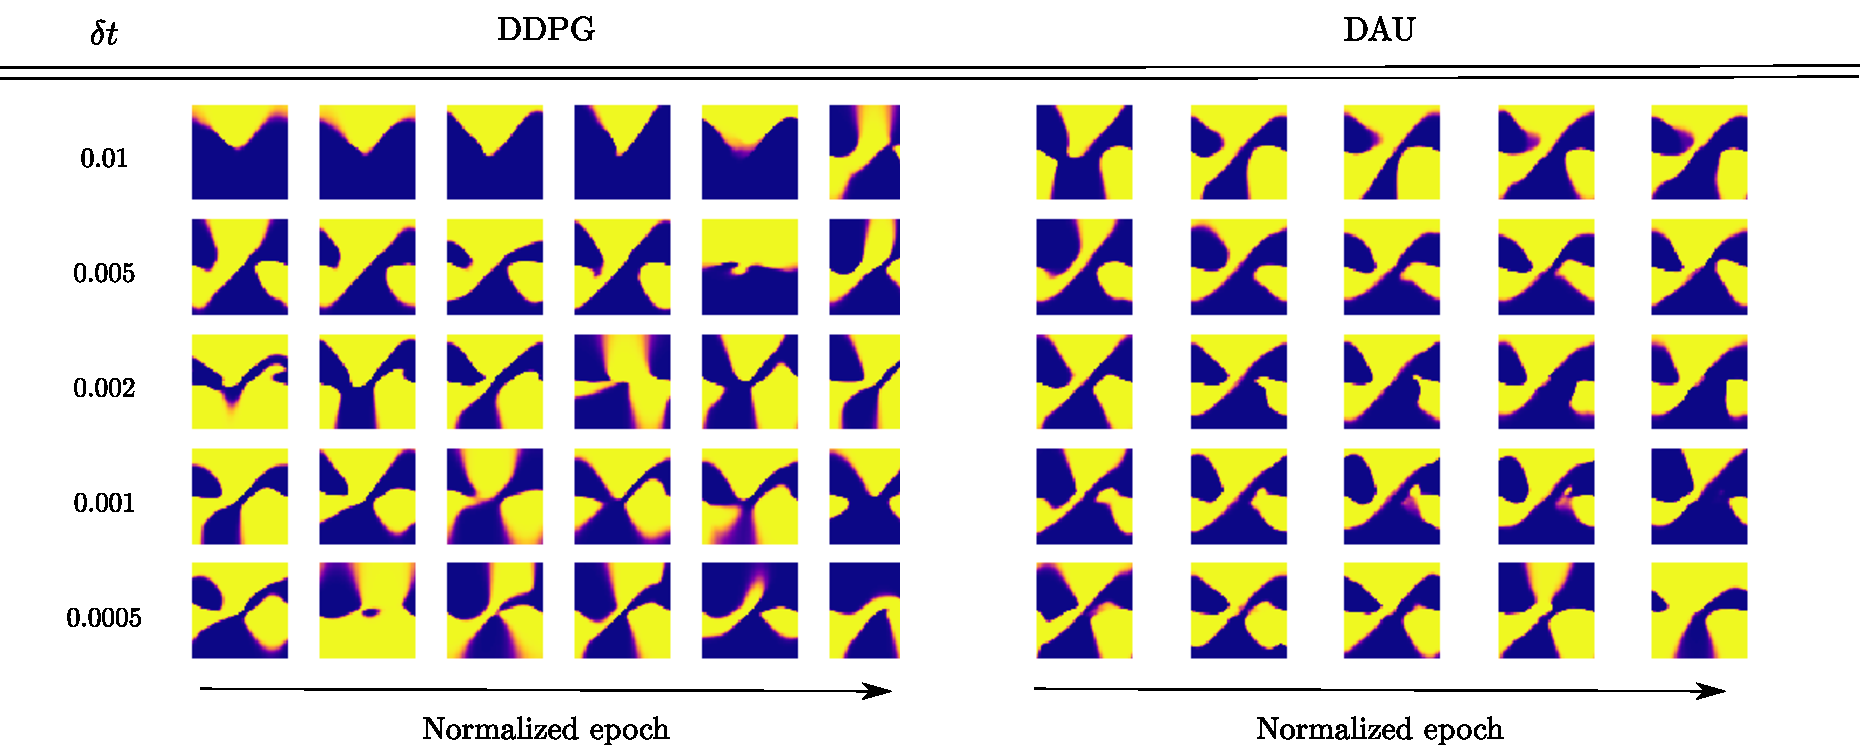
\includegraphics[width=\textwidth]{figs_data/pendulum_fig.pdf}
	\caption{Policies obtained by DDPG and AU at different macroscopic instants of training. Each image represents the policy learnt by the policy network, with $x$-axis representing angle, and $y$-axis angular velocity. The lighter the pixel, the closer to $1$ the action, the darker, the closer to $-1$.}
\end{figure*}

\TODO{
For the algorithm to admit a continuous-time limit, the discrete-time trajectories
of parameters must converge to well-defined trajectories as $\deltat$ goes to
$0$.
% The optimization steps should not be too large,
% in which case parameter trajectories could jump in a single gradient step,
% or too small, in which case the trajectories would become stationary as
% $\deltat$ goes to $0$.
This in turn imposes precise conditions on the scalings of the
learning rates.}% of algorithms robust to changes of the time discretization.  }

Informally, in the parameter updates
\eqref{eq:approx_deltaQ}--\eqref{eq:approx_bellman_A}, the quantity $\delta
Q_\deltat$ is of order $O(\deltat)$, because $s'=s+O(\deltat)$ in a
near-continuous system. Therefore, $\delta
Q_\deltat/\deltat$ is $O(1)$, so that the gradients used to
update $\theta$ and $\psi$ are $O(1)$. Therefore, if the
learning rates are of order $\deltat$, one would expect 
the parameters $\theta$ and $\psi$ to move by $O(\deltat)$ in
each time interval $\deltat$, thus hopefully converging to smooth
continuous-time trajectories. The next theorem formally confirms that
learning rates of order $\deltat$ are the only possibility.

% The updates of $\theta$ and $\psi$ are described in
% \eqref{eq:approx_bellman_A}.  To have parameter updates that do not explode or shrink to $0$ too
% fast as $\deltat \rightarrow 0$, both $\delta \theta$ and
% $\delta \psi$ should verify stochastic differential equations in the
% limit, and notably,
% have a deterministic component of order $\deltat$. As $\deltat$ goes to $0$,
% a Taylor expansion yields (with $\deltas\deq s'-s$)
% \begin{align}
% 	\delta Q_\deltat &= A(s, a)\,\deltat - r\,\deltat - \log(\gamma)
% 	\,V(s)\,\deltat - \partial_s V(s) \,\deltas\nonumber \\&- \frac{(\deltas)^T \partial_{s}^2 V(s) \deltas}{2} + \smallo\left(\deltat\right)\\
% 	\delta \theta_\deltat &= \eta^V_\deltat \partial_{\theta} V(s)
% 	\frac{\delta Q_\deltat}{\deltat} \\%+ \smallo\left(\eta^V_\deltat\right)\\
% 	\delta \psi_\deltat &= \eta^A_\deltat \partial_{\psi} A(s)
% 	\frac{\delta Q_\deltat}{\deltat} %+ \smallo\left(\eta^A_\deltat\right).
% \end{align}

% The next theorem confirms this analysis: with
% $\eta^V_\deltat = \alpha^V \deltat$ and $\eta^A_\deltat = \alpha^A
% \deltat$, the parameter updates follow a Euler discretization scheme
% for a continuous-time equation and have a well-defined limit behavior. On
% the other hand, with smaller learning rates the parameters do not move,
% and can explode instantaneously with larger learning rates.\TODO{keep? or
% just say "the next theorem confirms this"?}

\begin{theorem}
	\label{th:cont-params}
Let $(s_t,a_t)$ be some exploration trajectory in a near-continuous MDP. Set the learning rates to $\eta^V_\deltat =
\alpha^V \deltat^\beta$ and $\eta^A = \alpha^A \deltat^\beta$ for some
$\beta\geq 0$, and learn the parameters $\theta$ and $\psi$ by iterating
\eqref{eq:approx_deltaQ}--\eqref{eq:approx_bellman_A} along the
trajectory $(s_t,a_t)$. Then, when
$\deltat\to 0$:
% 	\TODO{Assume a continuous action space. Let $(s_t, a_t)_{t\geq 0}$ be a
% 	time continuous exploratory trajectory. Let $\pi$ be a sufficiently
% regular policy, and $\bar{A}$ and $\bar{V}$ be regular function approximators.}
% 	Let $\eta^V_\deltat = \alpha^V \deltat^\beta$ (resp. $\eta^A = \alpha^A \deltat^\beta$) be the learning rate
% 	of $V$ (resp. $\bar{A}$). Then, when learning on $(s_t, a_t)_{t\geq 0}$, 
	\begin{itemize}
		\item If $\beta = 1$ the discrete parameter trajectories converge to continuous parameter
			trajectories.% as $\deltat$ goes to $0$.
		\item If $\beta>1$ the parameters stay at their initial
		values.
		%trajectories become
		%stationary.% as $\deltat$ goes to $0$.
		\item If $\beta < 1$, the parameters can reach infinity
		in arbitrarily small physical time.%	parameters grow arbitrarily large in after an arbitrarily small physical time when $\deltat$ goes to $0$.
	\end{itemize}
\end{theorem}

% With this choice of learning rates, the limit SDEs are
% \begin{align}
% 	F &= A(s_t, a_t) - r_t - \log(\gamma) V(s_t) - \partial_s V(s_t) f(s_t, a_t)\nonumber\\
% 	G &= - \partial_s V(s_t, a_t) \Sigma(s_t, a_t)\nonumber\\
% 	d\theta_t &= (\alpha^V Fdt  + D \dbt)\partial_{\theta} V(s_t)\nonumber\\
% 	d\psi_t &= (\alpha^A Fdt  + D \dbt)\partial_{\psi} A(s_t, a_t)\nonumber.
% \end{align}

The resulting algorithm with suitable scalings,
\emph{Deep Advantage Updating} (DAU), is fully specified in Alg.~\ref{alg:dau} for
discrete actions, and in the supplementary material for continuous
actions.

%%% Local Variables:
%%% TeX-master: "icml_drau"
%%% End:



%! TEX root = icml_drau.tex
\section{Experiments}
\label{sec:exp}
%! TEX root = icml_drau.tex
\begin{figure*}[ht]
	\centering
	\includegraphics[width=\textwidth]{figs_data/full_results.pdf}
	\label{fig:full_results}
	\caption{Results on a variety of environments}
\end{figure*}

The experiment set provided here is specifically aimed at showing that
the proposed method DAU can operate efficiently on a wide range of time
discretizations, without specific tuning, while standard deep Q-learning
approaches cannot. DAU is compared to DDPG in continuous action settings and to DQN in
discrete action settings. \TODO{(We only test off-policy
algorithms.)}

In all experimental settings, we use the learning algorithm described in
alg.~\ref{alg:dau} and \TODO{supplementary, algo 1}. The variant of DDPG and DQN
used are described in the supplementary material, as well as all the hyperparameters
used. To make comparison fair, we still use rescaled discount factor $\gamma_\deltat$ and reward $r_\deltat$  as defined in equations \TODO{ref}, as well as scaled learning rates for DDPG and DQN.

Let us stress that quantities shown are rescaled to make comparison possible. For example,
return results are given in term of discretized return $R_\deltat$ as defined in Eq. \eqref{eq:discretized-return},\footnote{This mostly amounts to scaling rewards
by a factor $\deltat$ when this scaling is not naturally done in the environment. Environment specific
details are given in the supplementary material.} and, most notably, time elapsed is always given in
normalized epochs, i.e. the true number of epochs multiplied by the discretization timestep.


\paragraph{Qualitative experiments: Visualizing policies and values}
To provide qualitative results, and check that robustness to time
discretization is provided both in term of raw return results, but also in term
of convergence of approximate value function and policies, we first provide results on the simple pendulum environment
from the OpenAI Gym classic control suite.  This environment's state space is of dimension $2$. A visualization of both the learnt value and policy functions is obtained by plotting for each point of the phase diagram $(\theta, \dot{\theta})$ its value and policy. results are presented in
Fig.~\ref{fig:pend} for the policy function and in Fig.\TODO{ref} in Supplementary \TODO{ref} for the value function.

We observe the learnt policy at several instants in physical time (or normalized epochs) during training, for various time discretizations $\deltat$, for both DAU and DDPG. With DAU, the agent's policy quickly converges for every time discretization without specific hyperparameter tuning. On the contrary, with DDPG, the agent is only able to learn for the two highest time discretization, and learning gets harder as $\deltat$ decreases.

\paragraph{Quantitative experiments}
We benchmark DAU against DDPG on classic control benchmarks: Pendulum, Cartpole, BipedalWalker, Ant and Half-Cheetah environments from OpenAI Gym. For Pendulum and Ant, DDPG is able to learn for the highest $\deltat$ but fails for the others, while DAU remains reasonably invariant to the time discretization. On Bipedal Walker, DDPG is never able to learn while DAU is achieving decent performance for all the $\deltat$'s. On Cartpole and Half Cheetah, results are less clear. On Cartpole, noise dominates, which makes interpretation difficult. On Half Cheetah, DAU is not clearly more invariant to time discretization than DDPG. This could be explained by the multiple suboptimal regimes that coexist in the half cheetah environment (walking on the head, walking on the back), and that DAU may fail to correctly weight the performance of each regime (as explained in Section \ref{sec:discussions}).

% \begin{figure}[h]
%   \centering
%   \includegraphics[width=\columnwidth]{figs_data/cartpole_lc.png}
%   \caption{Cartpole}
%   \label{fig:cartpole-lc}
% \end{figure}

% \begin{figure}[h]
%   \centering
%   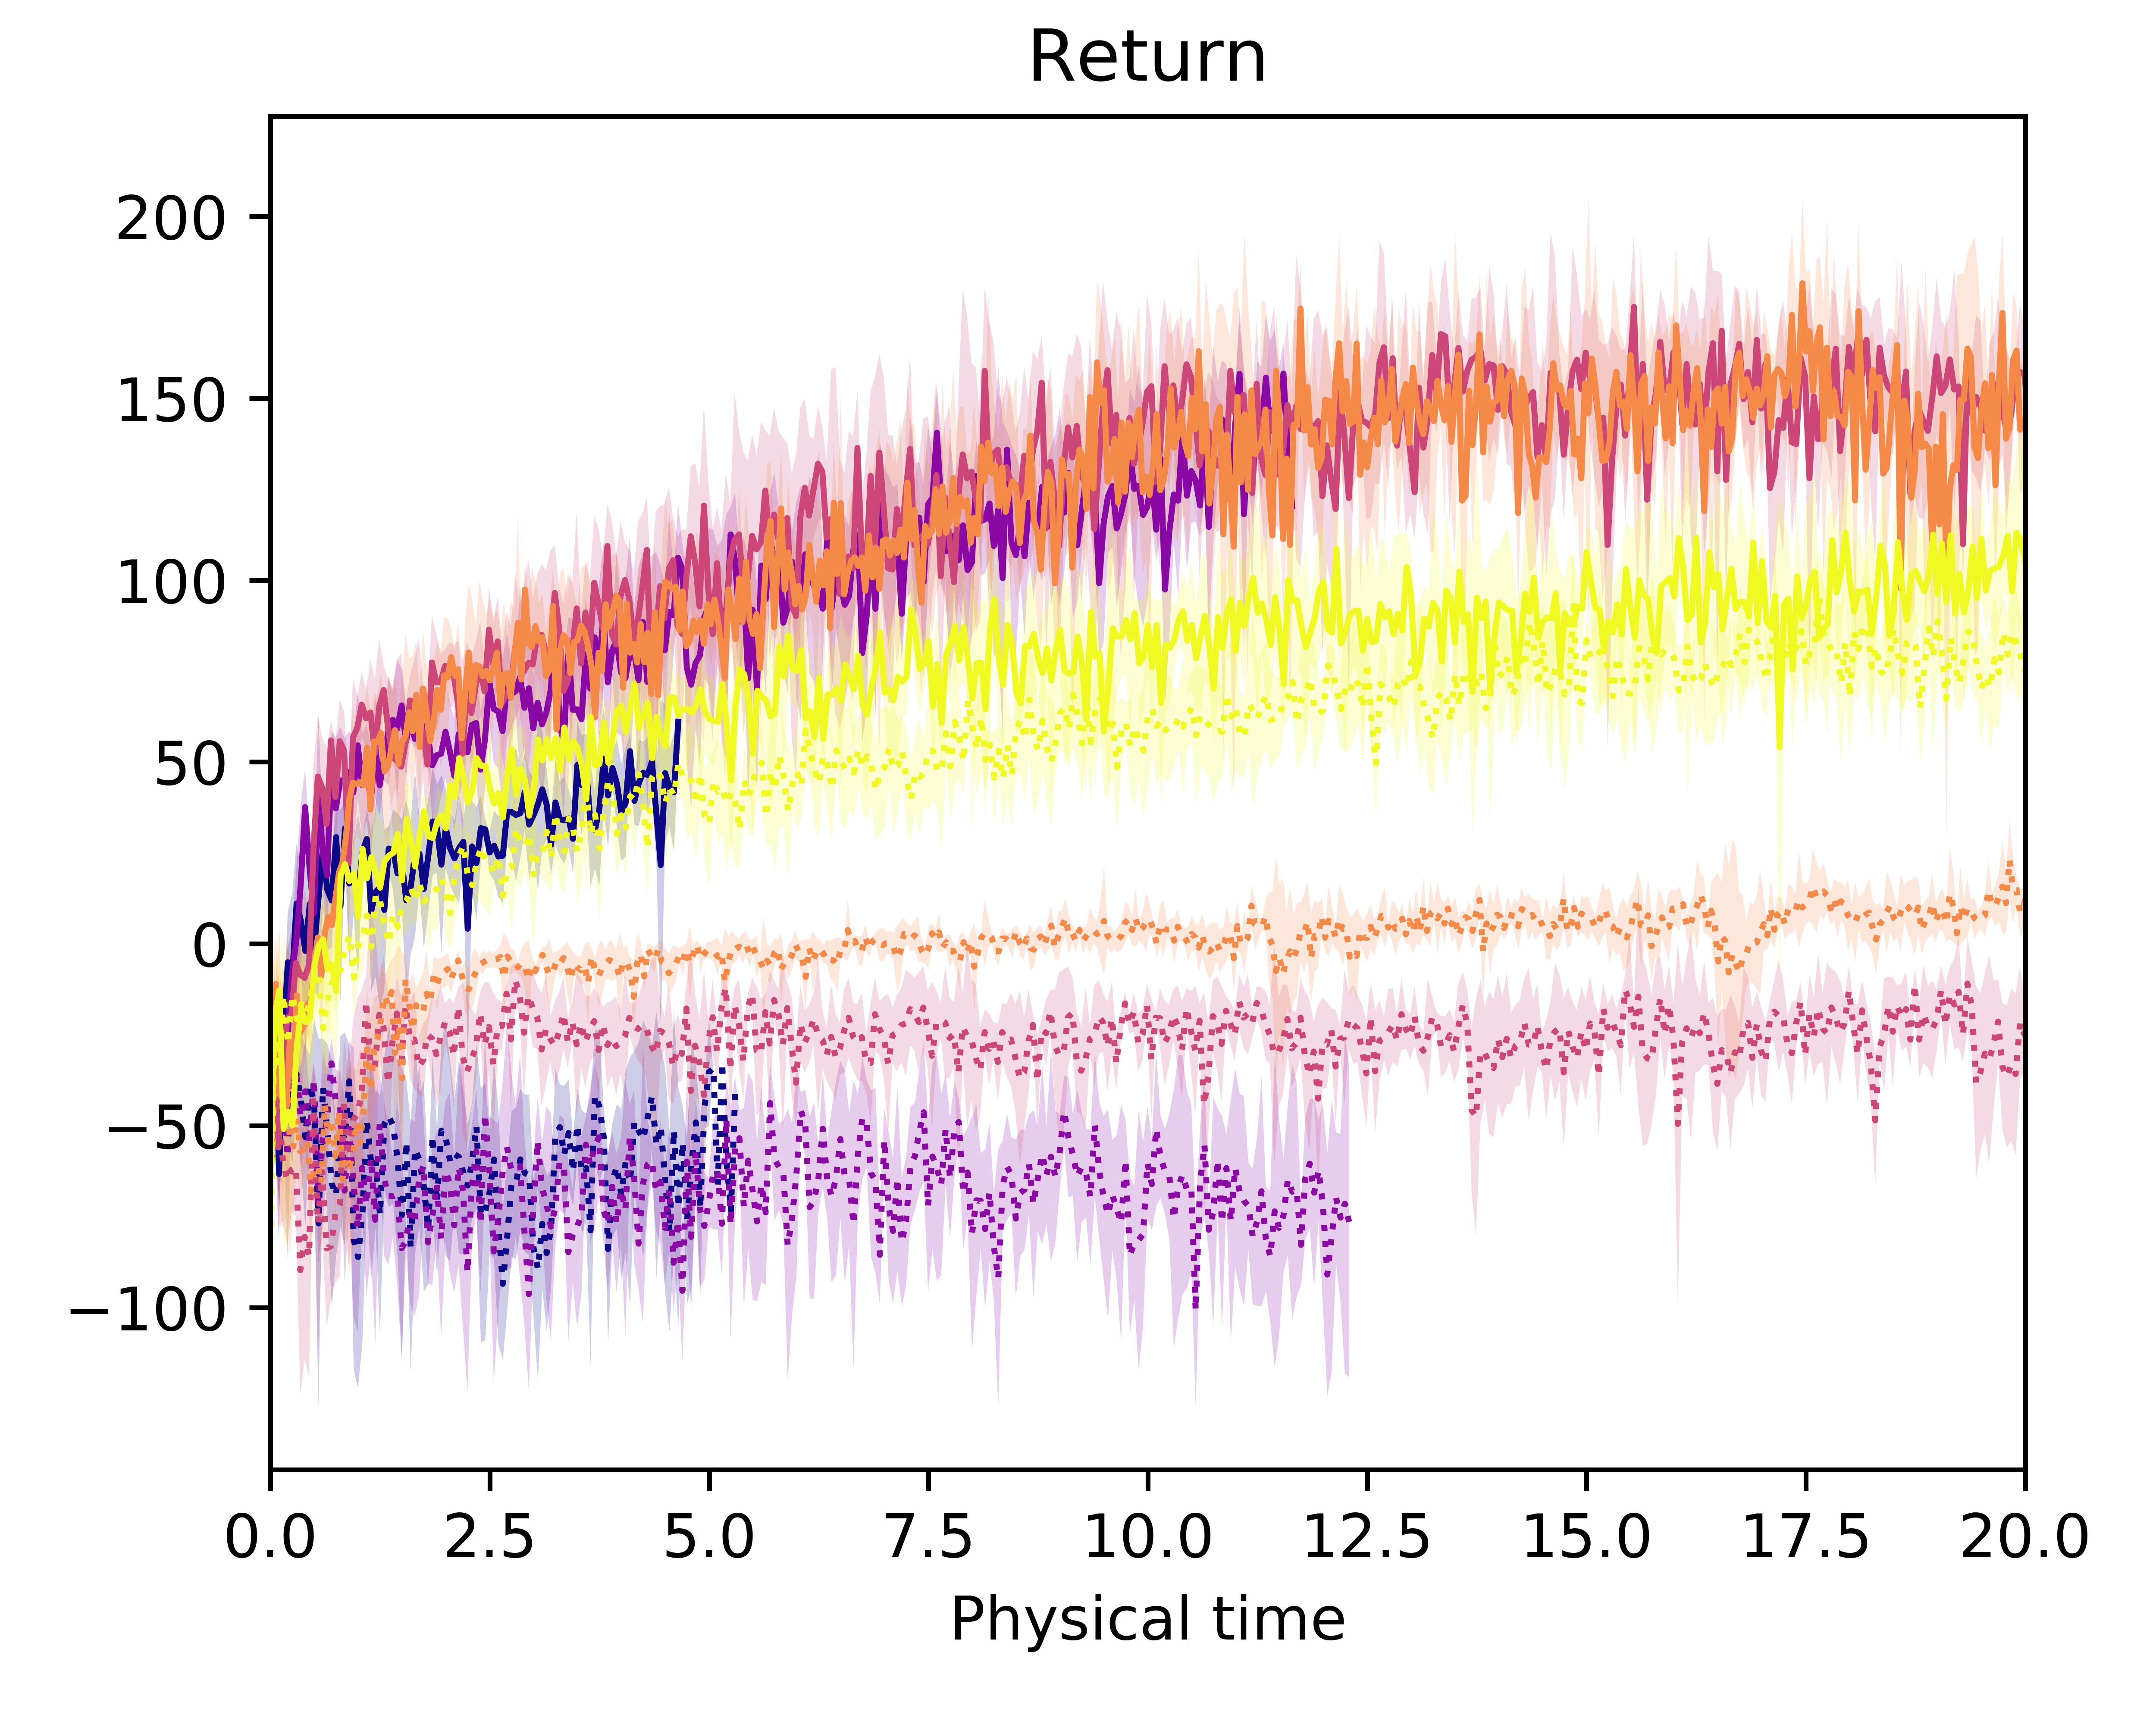
\includegraphics[width=\columnwidth]{figs_data/ant_lc.png}
%   \caption{Ant}
%   \label{fig:ant-lc}
% \end{figure}
% 
% \begin{figure}[h]
%   \centering
%   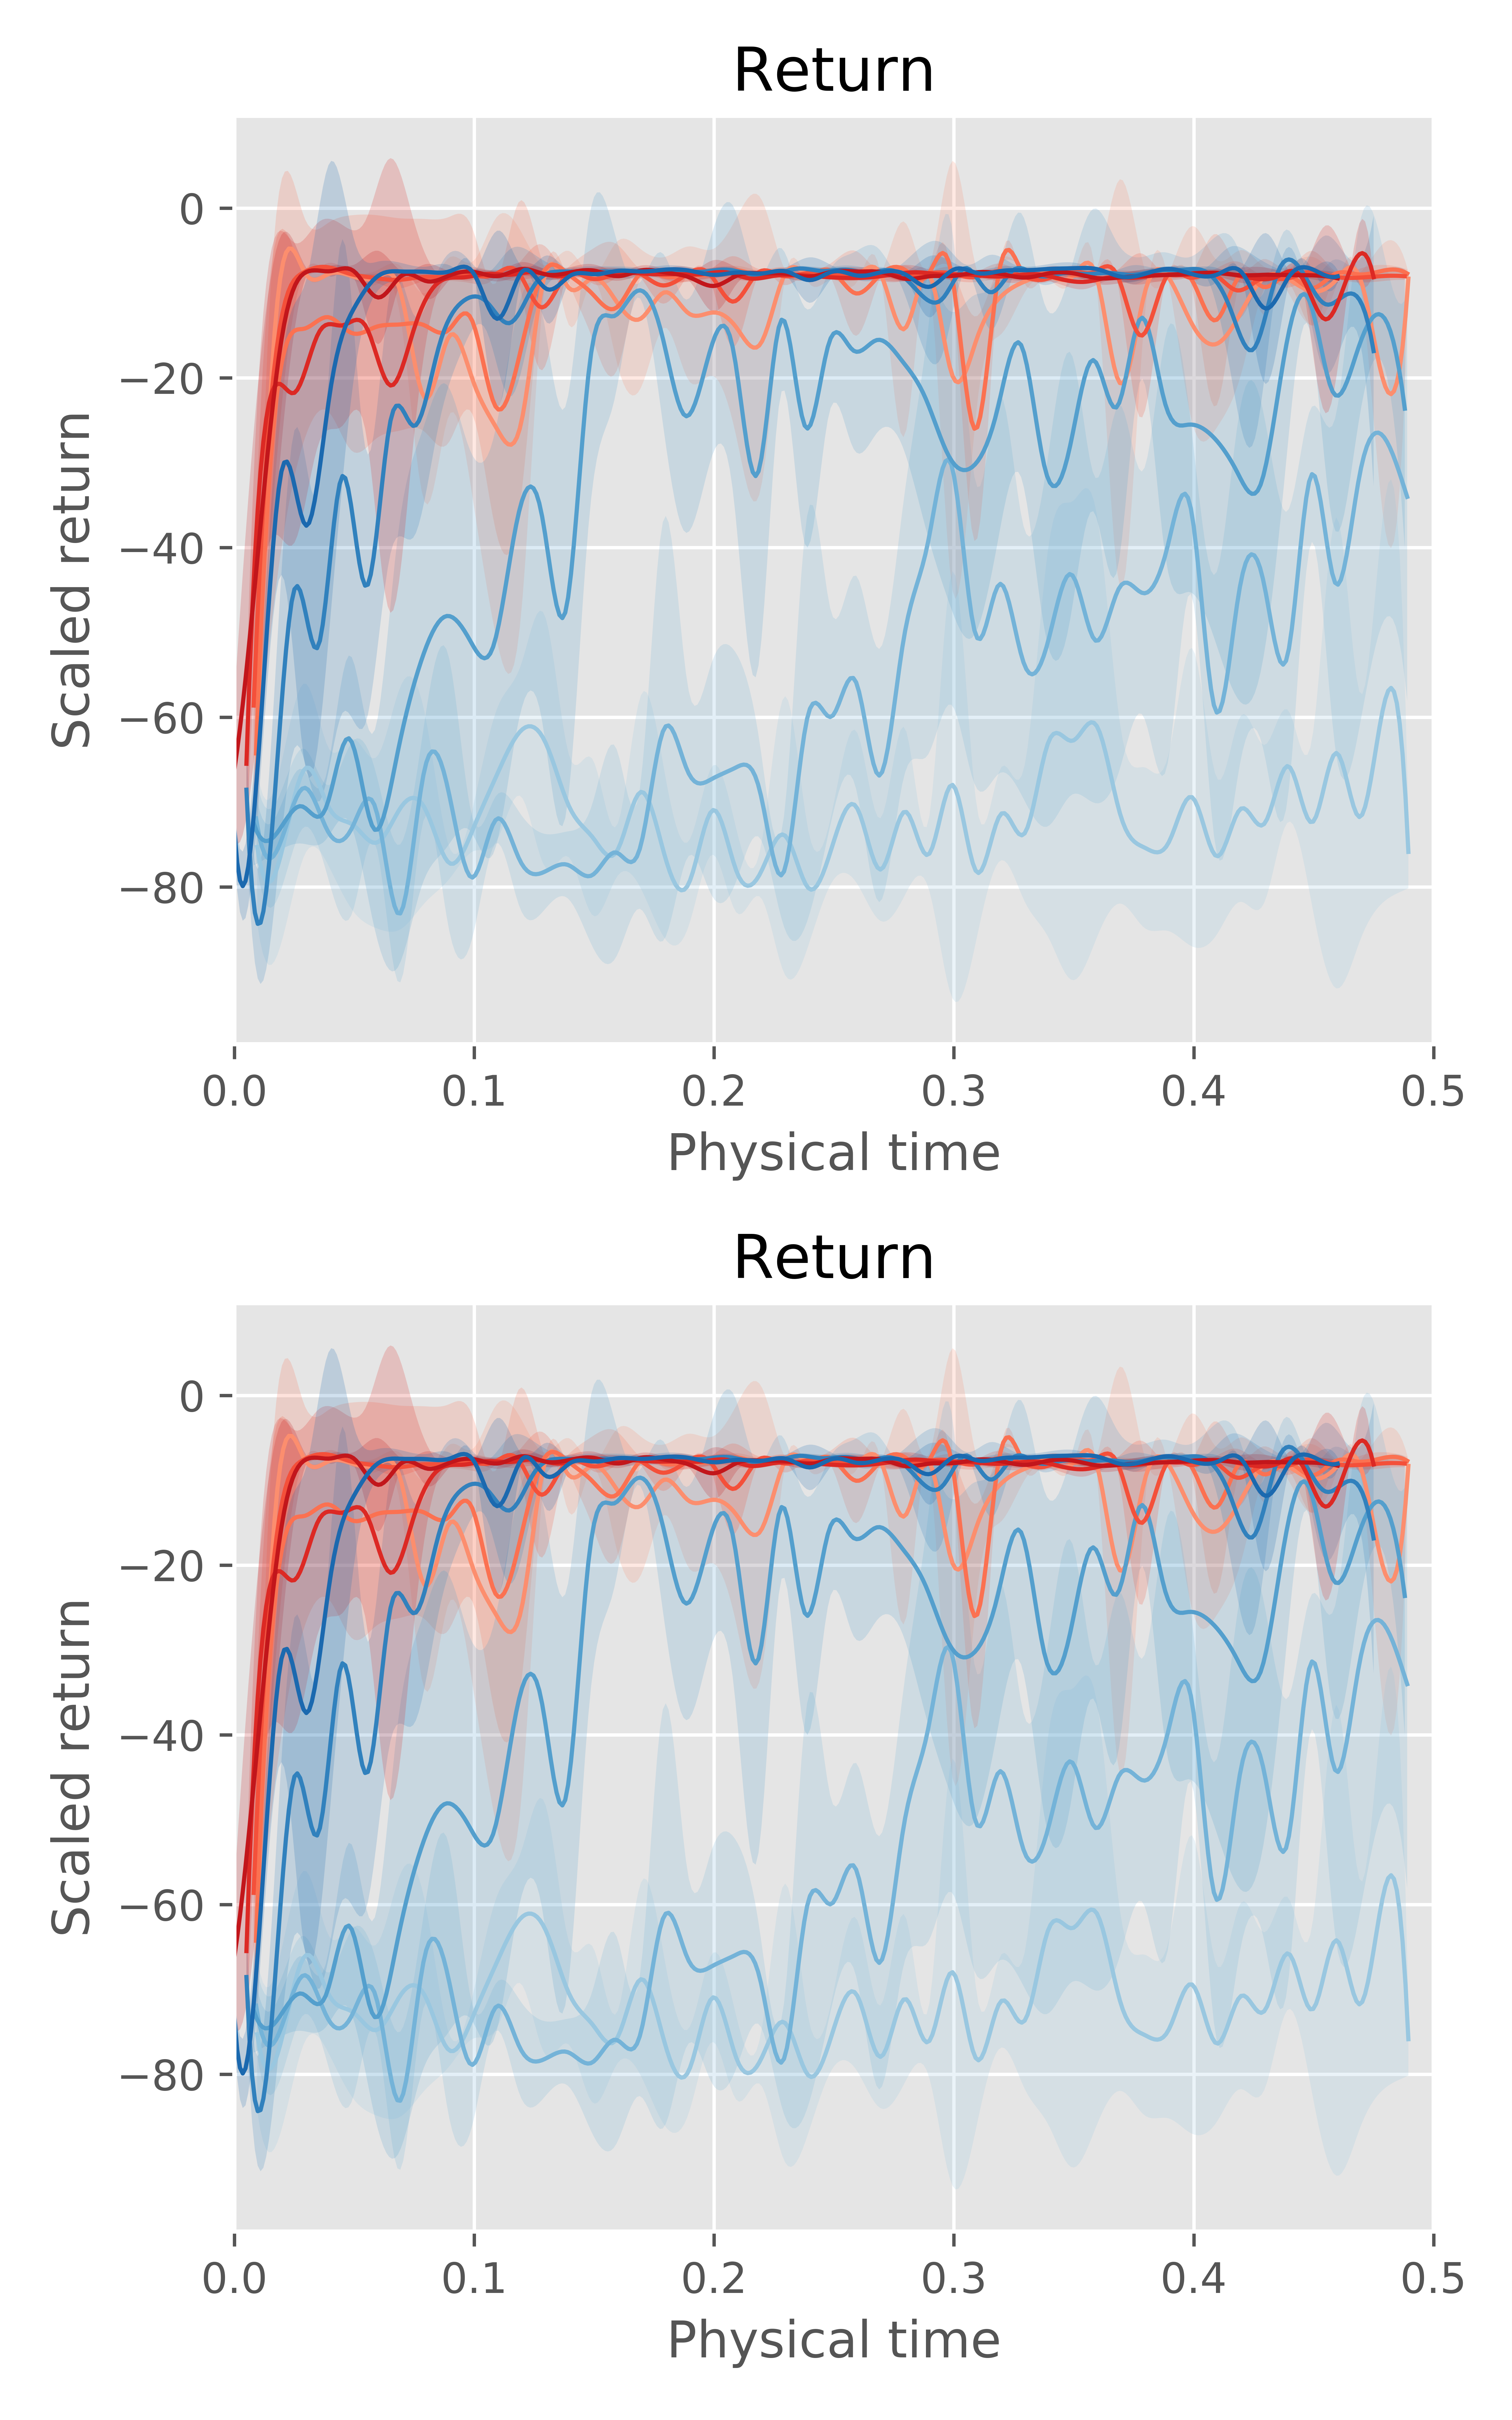
\includegraphics[width=\columnwidth]{figs_data/pendulum_lc.png}
%   \caption{Pendulum}
%   \label{fig:pendulum-lc}
% \end{figure}


\section{Discussions}

TODO


%! TEX root = icml_drau.tex
\section{Conclusion}



From the observation that standard Q-learning based methods fail to learn with small time discretization,
we derived a formal explanation for their sensitiviy.
% Empirically, we find that
% Q-learning-based approaches such as
% \emph{Deep Q-learning}~\cite{dqn} and \emph{Deep Deterministic
% Policy Gradient}~\cite{ddpg} 
% are highly sensitive to variations of time discretization and
% collapse with small time steps. Formally, we prove that
% $Q$-learning does not exist in
% continuous time.
We defined an off-policy algorithm based on this analysis which yields better robustness properties.



\bibliography{icml_drau.bib}
\bibliographystyle{icml2018}
\end{document}


% This document was modified from the file originally made available by
% Pat Langley and Andrea Danyluk for ICML-2K. This version was created
% by Iain Murray in 2018. It was modified from a version from Dan Roy in
% 2017, which was based on a version from Lise Getoor and Tobias
% Scheffer, which was slightly modified from the 2010 version by
% Thorsten Joachims & Johannes Fuernkranz, slightly modified from the
% 2009 version by Kiri Wagstaff and Sam Roweis's 2008 version, which is
% slightly modified from Prasad Tadepalli's 2007 version which is a
% lightly changed version of the previous year's version by Andrew
% Moore, which was in turn edited from those of Kristian Kersting and
% Codrina Lauth. Alex Smola contributed to the algorithmic style files.
